\documentclass[twoside]{book}

% Packages required by doxygen
\usepackage{fixltx2e}
\usepackage{calc}
\usepackage{doxygen}
\usepackage[export]{adjustbox} % also loads graphicx
\usepackage{graphicx}
\usepackage[utf8]{inputenc}
\usepackage{makeidx}
\usepackage{multicol}
\usepackage{multirow}
\PassOptionsToPackage{warn}{textcomp}
\usepackage{textcomp}
\usepackage[nointegrals]{wasysym}
\usepackage[table]{xcolor}

% Font selection
\usepackage[T1]{fontenc}
\usepackage[scaled=.90]{helvet}
\usepackage{courier}
\usepackage{amssymb}
\usepackage{sectsty}
\renewcommand{\familydefault}{\sfdefault}
\allsectionsfont{%
  \fontseries{bc}\selectfont%
  \color{darkgray}%
}
\renewcommand{\DoxyLabelFont}{%
  \fontseries{bc}\selectfont%
  \color{darkgray}%
}
\newcommand{\+}{\discretionary{\mbox{\scriptsize$\hookleftarrow$}}{}{}}

% Page & text layout
\usepackage{geometry}
\geometry{%
  a4paper,%
  top=2.5cm,%
  bottom=2.5cm,%
  left=2.5cm,%
  right=2.5cm%
}
\tolerance=750
\hfuzz=15pt
\hbadness=750
\setlength{\emergencystretch}{15pt}
\setlength{\parindent}{0cm}
\setlength{\parskip}{3ex plus 2ex minus 2ex}
\makeatletter
\renewcommand{\paragraph}{%
  \@startsection{paragraph}{4}{0ex}{-1.0ex}{1.0ex}{%
    \normalfont\normalsize\bfseries\SS@parafont%
  }%
}
\renewcommand{\subparagraph}{%
  \@startsection{subparagraph}{5}{0ex}{-1.0ex}{1.0ex}{%
    \normalfont\normalsize\bfseries\SS@subparafont%
  }%
}
\makeatother

% Headers & footers
\usepackage{fancyhdr}
\pagestyle{fancyplain}
\fancyhead[LE]{\fancyplain{}{\bfseries\thepage}}
\fancyhead[CE]{\fancyplain{}{}}
\fancyhead[RE]{\fancyplain{}{\bfseries\leftmark}}
\fancyhead[LO]{\fancyplain{}{\bfseries\rightmark}}
\fancyhead[CO]{\fancyplain{}{}}
\fancyhead[RO]{\fancyplain{}{\bfseries\thepage}}
\fancyfoot[LE]{\fancyplain{}{}}
\fancyfoot[CE]{\fancyplain{}{}}
\fancyfoot[RE]{\fancyplain{}{\bfseries\scriptsize Generated by Doxygen }}
\fancyfoot[LO]{\fancyplain{}{\bfseries\scriptsize Generated by Doxygen }}
\fancyfoot[CO]{\fancyplain{}{}}
\fancyfoot[RO]{\fancyplain{}{}}
\renewcommand{\footrulewidth}{0.4pt}
\renewcommand{\chaptermark}[1]{%
  \markboth{#1}{}%
}
\renewcommand{\sectionmark}[1]{%
  \markright{\thesection\ #1}%
}

% Indices & bibliography
\usepackage{natbib}
\usepackage[titles]{tocloft}
\setcounter{tocdepth}{3}
\setcounter{secnumdepth}{5}
\makeindex

% Hyperlinks (required, but should be loaded last)
\usepackage{ifpdf}
\ifpdf
  \usepackage[pdftex,pagebackref=true]{hyperref}
\else
  \usepackage[ps2pdf,pagebackref=true]{hyperref}
\fi
\hypersetup{%
  colorlinks=true,%
  linkcolor=blue,%
  citecolor=blue,%
  unicode%
}

% Custom commands
\newcommand{\clearemptydoublepage}{%
  \newpage{\pagestyle{empty}\cleardoublepage}%
}

\usepackage{caption}
\captionsetup{labelsep=space,justification=centering,font={bf},singlelinecheck=off,skip=4pt,position=top}

%===== C O N T E N T S =====

\begin{document}

% Titlepage & ToC
\hypersetup{pageanchor=false,
             bookmarksnumbered=true,
             pdfencoding=unicode
            }
\pagenumbering{roman}
\begin{titlepage}
\vspace*{7cm}
\begin{center}%
{\Large A\+VL Tree \\[1ex]\large 1.\+0.\+0 }\\
\vspace*{1cm}
{\large Generated by Doxygen 1.8.11}\\
\end{center}
\end{titlepage}
\clearemptydoublepage
\tableofcontents
\clearemptydoublepage
\pagenumbering{arabic}
\hypersetup{pageanchor=true}

%--- Begin generated contents ---
\chapter{Class Index}
\section{Class List}
Here are the classes, structs, unions and interfaces with brief descriptions\+:\begin{DoxyCompactList}
\item\contentsline{section}{\hyperlink{class_a_v_l___tree}{A\+V\+L\+\_\+\+Tree$<$ T $>$} \\*A\+VL Tree class }{\pageref{class_a_v_l___tree}}{}
\item\contentsline{section}{\hyperlink{class_logger}{Logger} }{\pageref{class_logger}}{}
\item\contentsline{section}{\hyperlink{class_node}{Node$<$ T $>$} \\*A\+VL \hyperlink{class_node}{Node} class }{\pageref{class_node}}{}
\end{DoxyCompactList}

\chapter{File Index}
\section{File List}
Here is a list of all files with brief descriptions\+:\begin{DoxyCompactList}
\item\contentsline{section}{/home/kacper/\+Pulpit/\+P\+A\+M\+S\+I -\/ Projekty/\+Projekt 1/prj/\hyperlink{main_8cpp}{main.\+cpp} }{\pageref{main_8cpp}}{}
\item\contentsline{section}{/home/kacper/\+Pulpit/\+P\+A\+M\+S\+I -\/ Projekty/\+Projekt 1/prj/inc/\hyperlink{additional_functions_8hpp}{additional\+Functions.\+hpp} }{\pageref{additional_functions_8hpp}}{}
\item\contentsline{section}{/home/kacper/\+Pulpit/\+P\+A\+M\+S\+I -\/ Projekty/\+Projekt 1/prj/inc/\hyperlink{_a_v_l___tree_8hpp}{A\+V\+L\+\_\+\+Tree.\+hpp} }{\pageref{_a_v_l___tree_8hpp}}{}
\item\contentsline{section}{/home/kacper/\+Pulpit/\+P\+A\+M\+S\+I -\/ Projekty/\+Projekt 1/prj/inc/\hyperlink{logger_8hpp}{logger.\+hpp} }{\pageref{logger_8hpp}}{}
\item\contentsline{section}{/home/kacper/\+Pulpit/\+P\+A\+M\+S\+I -\/ Projekty/\+Projekt 1/prj/inc/\hyperlink{node_8hpp}{node.\+hpp} }{\pageref{node_8hpp}}{}
\item\contentsline{section}{/home/kacper/\+Pulpit/\+P\+A\+M\+S\+I -\/ Projekty/\+Projekt 1/prj/src/\hyperlink{logger_8cpp}{logger.\+cpp} }{\pageref{logger_8cpp}}{}
\end{DoxyCompactList}

\chapter{Class Documentation}
\hypertarget{class_a_v_l___tree}{}\section{A\+V\+L\+\_\+\+Tree$<$ T $>$ Class Template Reference}
\label{class_a_v_l___tree}\index{A\+V\+L\+\_\+\+Tree$<$ T $>$@{A\+V\+L\+\_\+\+Tree$<$ T $>$}}


A\+VL Tree class.  




{\ttfamily \#include $<$A\+V\+L\+\_\+\+Tree.\+hpp$>$}

\subsection*{Public Member Functions}
\begin{DoxyCompactItemize}
\item 
\hyperlink{class_a_v_l___tree_a129151ce51f97168c7cd9c84a6b17500}{A\+V\+L\+\_\+\+Tree} ()
\item 
\hyperlink{class_a_v_l___tree_a082bb7b47a8351639059e7063b97a114}{$\sim$\+A\+V\+L\+\_\+\+Tree} ()
\item 
int \hyperlink{class_a_v_l___tree_a74bbdd68e0767102ed33dc9253a76b7e}{height} ()
\item 
int \hyperlink{class_a_v_l___tree_ab865e8048400cb149e11f4bcb5c6f9b2}{size} ()
\item 
bool \hyperlink{class_a_v_l___tree_a2384f725aba6caf38392b77414514815}{contains} (T value)
\item 
bool \hyperlink{class_a_v_l___tree_a95d4d0b742c901ba78fcb2e5a91fed08}{insert} (T value)
\item 
bool \hyperlink{class_a_v_l___tree_a08b1c0b73d635728ea024edf0748e13d}{delete\+Value} (T value)
\item 
bool \hyperlink{class_a_v_l___tree_a2dbb95af3faf3933837ceeb478dd718f}{print\+Tree\+Pre\+Order} ()
\begin{DoxyCompactList}\small\item\em Public method that shows tree structure. \end{DoxyCompactList}\item 
bool \hyperlink{class_a_v_l___tree_a1bffe71cf2c76fa3edf66a2357ae3bc6}{print\+Tree\+In\+Order} ()
\begin{DoxyCompactList}\small\item\em Public method that shows tree structure. \end{DoxyCompactList}\item 
bool \hyperlink{class_a_v_l___tree_a4641e4bcc182de5bcd72424def3e92c1}{print\+Tree\+Post\+Order} ()
\begin{DoxyCompactList}\small\item\em Public method that shows tree structure. \end{DoxyCompactList}\end{DoxyCompactItemize}


\subsection{Detailed Description}
\subsubsection*{template$<$class T$>$\\*
class A\+V\+L\+\_\+\+Tree$<$ T $>$}

A\+VL Tree class. 

Class that represents algorithm of A\+VL Tree. It contains pointer to root \hyperlink{class_node}{Node}, node count, and methods to work with A\+VL Nodes/\+Trees 

Definition at line 21 of file A\+V\+L\+\_\+\+Tree.\+hpp.



\subsection{Constructor \& Destructor Documentation}
\index{A\+V\+L\+\_\+\+Tree@{A\+V\+L\+\_\+\+Tree}!A\+V\+L\+\_\+\+Tree@{A\+V\+L\+\_\+\+Tree}}
\index{A\+V\+L\+\_\+\+Tree@{A\+V\+L\+\_\+\+Tree}!A\+V\+L\+\_\+\+Tree@{A\+V\+L\+\_\+\+Tree}}
\subsubsection[{\texorpdfstring{A\+V\+L\+\_\+\+Tree()}{AVL_Tree()}}]{\setlength{\rightskip}{0pt plus 5cm}template$<$class T$>$ {\bf A\+V\+L\+\_\+\+Tree}$<$ T $>$\+::{\bf A\+V\+L\+\_\+\+Tree} (
\begin{DoxyParamCaption}
{}
\end{DoxyParamCaption}
)\hspace{0.3cm}{\ttfamily [inline]}}\hypertarget{class_a_v_l___tree_a129151ce51f97168c7cd9c84a6b17500}{}\label{class_a_v_l___tree_a129151ce51f97168c7cd9c84a6b17500}
Constructor creates new \hyperlink{class_a_v_l___tree}{A\+V\+L\+\_\+\+Tree} with it\textquotesingle{}s root set to null 

Definition at line 212 of file A\+V\+L\+\_\+\+Tree.\+hpp.

\index{A\+V\+L\+\_\+\+Tree@{A\+V\+L\+\_\+\+Tree}!````~A\+V\+L\+\_\+\+Tree@{$\sim$\+A\+V\+L\+\_\+\+Tree}}
\index{````~A\+V\+L\+\_\+\+Tree@{$\sim$\+A\+V\+L\+\_\+\+Tree}!A\+V\+L\+\_\+\+Tree@{A\+V\+L\+\_\+\+Tree}}
\subsubsection[{\texorpdfstring{$\sim$\+A\+V\+L\+\_\+\+Tree()}{~AVL_Tree()}}]{\setlength{\rightskip}{0pt plus 5cm}template$<$class T$>$ {\bf A\+V\+L\+\_\+\+Tree}$<$ T $>$\+::$\sim${\bf A\+V\+L\+\_\+\+Tree} (
\begin{DoxyParamCaption}
{}
\end{DoxyParamCaption}
)\hspace{0.3cm}{\ttfamily [inline]}}\hypertarget{class_a_v_l___tree_a082bb7b47a8351639059e7063b97a114}{}\label{class_a_v_l___tree_a082bb7b47a8351639059e7063b97a114}
Destructor for A\+VL Tree -\/ it destructs all of the nodes by recursion 

Definition at line 215 of file A\+V\+L\+\_\+\+Tree.\+hpp.



\subsection{Member Function Documentation}
\index{A\+V\+L\+\_\+\+Tree@{A\+V\+L\+\_\+\+Tree}!contains@{contains}}
\index{contains@{contains}!A\+V\+L\+\_\+\+Tree@{A\+V\+L\+\_\+\+Tree}}
\subsubsection[{\texorpdfstring{contains(\+T value)}{contains(T value)}}]{\setlength{\rightskip}{0pt plus 5cm}template$<$class T $>$ bool {\bf A\+V\+L\+\_\+\+Tree}$<$ T $>$\+::contains (
\begin{DoxyParamCaption}
\item[{T}]{value}
\end{DoxyParamCaption}
)}\hypertarget{class_a_v_l___tree_a2384f725aba6caf38392b77414514815}{}\label{class_a_v_l___tree_a2384f725aba6caf38392b77414514815}
Public method calls contains(\+Node$<$\+T$>$$\ast$ node, T value) private method in order to always start searching for a value in root node\+:
\begin{DoxyItemize}
\item if value doesn\textquotesingle{}t exist in the tree it returns false
\item if value already exists in the tree returns true 
\begin{DoxyParams}{Parameters}
{\em value} & -\/ value that program will search in the tree \\
\hline
\end{DoxyParams}

\end{DoxyItemize}

Definition at line 316 of file A\+V\+L\+\_\+\+Tree.\+hpp.

\index{A\+V\+L\+\_\+\+Tree@{A\+V\+L\+\_\+\+Tree}!delete\+Value@{delete\+Value}}
\index{delete\+Value@{delete\+Value}!A\+V\+L\+\_\+\+Tree@{A\+V\+L\+\_\+\+Tree}}
\subsubsection[{\texorpdfstring{delete\+Value(\+T value)}{deleteValue(T value)}}]{\setlength{\rightskip}{0pt plus 5cm}template$<$class T $>$ bool {\bf A\+V\+L\+\_\+\+Tree}$<$ T $>$\+::delete\+Value (
\begin{DoxyParamCaption}
\item[{T}]{value}
\end{DoxyParamCaption}
)}\hypertarget{class_a_v_l___tree_a08b1c0b73d635728ea024edf0748e13d}{}\label{class_a_v_l___tree_a08b1c0b73d635728ea024edf0748e13d}
Public method that removes node with selected value. First it validate if value which has to be removed is not null, then it validates if value exists in the tree. If value exists, then private method delete\+Value(\+Node$<$\+T$>$ node, T value) is called and it decrements node\+Count value\+:
\begin{DoxyItemize}
\item if value does not exists in the tree, or value is null it returns false
\item if value exist in the tree it returns true once value is removed 
\begin{DoxyParams}{Parameters}
{\em value} & -\/ value to delete \\
\hline
\end{DoxyParams}

\end{DoxyItemize}

Definition at line 451 of file A\+V\+L\+\_\+\+Tree.\+hpp.

\index{A\+V\+L\+\_\+\+Tree@{A\+V\+L\+\_\+\+Tree}!height@{height}}
\index{height@{height}!A\+V\+L\+\_\+\+Tree@{A\+V\+L\+\_\+\+Tree}}
\subsubsection[{\texorpdfstring{height()}{height()}}]{\setlength{\rightskip}{0pt plus 5cm}template$<$class T $>$ int {\bf A\+V\+L\+\_\+\+Tree}$<$ T $>$\+::height (
\begin{DoxyParamCaption}
{}
\end{DoxyParamCaption}
)}\hypertarget{class_a_v_l___tree_a74bbdd68e0767102ed33dc9253a76b7e}{}\label{class_a_v_l___tree_a74bbdd68e0767102ed33dc9253a76b7e}
Method for test purposes, it returns height of the tree 

Definition at line 283 of file A\+V\+L\+\_\+\+Tree.\+hpp.

\index{A\+V\+L\+\_\+\+Tree@{A\+V\+L\+\_\+\+Tree}!insert@{insert}}
\index{insert@{insert}!A\+V\+L\+\_\+\+Tree@{A\+V\+L\+\_\+\+Tree}}
\subsubsection[{\texorpdfstring{insert(\+T value)}{insert(T value)}}]{\setlength{\rightskip}{0pt plus 5cm}template$<$class T $>$ bool {\bf A\+V\+L\+\_\+\+Tree}$<$ T $>$\+::insert (
\begin{DoxyParamCaption}
\item[{T}]{value}
\end{DoxyParamCaption}
)}\hypertarget{class_a_v_l___tree_a95d4d0b742c901ba78fcb2e5a91fed08}{}\label{class_a_v_l___tree_a95d4d0b742c901ba78fcb2e5a91fed08}
Public method that inserts value to the A\+VL tree. First it validate if given value already exists in the tree. If not method calls private method insert(\+Node$<$\+T$>$$\ast$ node, T value) and increments node\+Count\+:
\begin{DoxyItemize}
\item if value already exists in the tree, or value is null it returns false
\item if value doesn\textquotesingle{}t exist in the tree it returns true 
\begin{DoxyParams}{Parameters}
{\em value} & -\/ value that program inserts \\
\hline
\end{DoxyParams}

\end{DoxyItemize}

Definition at line 342 of file A\+V\+L\+\_\+\+Tree.\+hpp.

\index{A\+V\+L\+\_\+\+Tree@{A\+V\+L\+\_\+\+Tree}!print\+Tree\+In\+Order@{print\+Tree\+In\+Order}}
\index{print\+Tree\+In\+Order@{print\+Tree\+In\+Order}!A\+V\+L\+\_\+\+Tree@{A\+V\+L\+\_\+\+Tree}}
\subsubsection[{\texorpdfstring{print\+Tree\+In\+Order()}{printTreeInOrder()}}]{\setlength{\rightskip}{0pt plus 5cm}template$<$class T $>$ bool {\bf A\+V\+L\+\_\+\+Tree}$<$ T $>$\+::print\+Tree\+In\+Order (
\begin{DoxyParamCaption}
{}
\end{DoxyParamCaption}
)}\hypertarget{class_a_v_l___tree_a1bffe71cf2c76fa3edf66a2357ae3bc6}{}\label{class_a_v_l___tree_a1bffe71cf2c76fa3edf66a2357ae3bc6}


Public method that shows tree structure. 

Public method that calls private method print\+Tree\+Order(\+Node$<$\+T$>$$\ast$ node) if root exists.
\begin{DoxyItemize}
\item returns false if root is null
\item returns status of called method (true or false) 
\end{DoxyItemize}

Definition at line 551 of file A\+V\+L\+\_\+\+Tree.\+hpp.

\index{A\+V\+L\+\_\+\+Tree@{A\+V\+L\+\_\+\+Tree}!print\+Tree\+Post\+Order@{print\+Tree\+Post\+Order}}
\index{print\+Tree\+Post\+Order@{print\+Tree\+Post\+Order}!A\+V\+L\+\_\+\+Tree@{A\+V\+L\+\_\+\+Tree}}
\subsubsection[{\texorpdfstring{print\+Tree\+Post\+Order()}{printTreePostOrder()}}]{\setlength{\rightskip}{0pt plus 5cm}template$<$class T $>$ bool {\bf A\+V\+L\+\_\+\+Tree}$<$ T $>$\+::print\+Tree\+Post\+Order (
\begin{DoxyParamCaption}
{}
\end{DoxyParamCaption}
)}\hypertarget{class_a_v_l___tree_a4641e4bcc182de5bcd72424def3e92c1}{}\label{class_a_v_l___tree_a4641e4bcc182de5bcd72424def3e92c1}


Public method that shows tree structure. 

Public method that calls private method print\+Tree\+Order(\+Node$<$\+T$>$$\ast$ node) if root exists.
\begin{DoxyItemize}
\item returns false if root is null
\item returns status of called method (true or false) 
\end{DoxyItemize}

Definition at line 575 of file A\+V\+L\+\_\+\+Tree.\+hpp.

\index{A\+V\+L\+\_\+\+Tree@{A\+V\+L\+\_\+\+Tree}!print\+Tree\+Pre\+Order@{print\+Tree\+Pre\+Order}}
\index{print\+Tree\+Pre\+Order@{print\+Tree\+Pre\+Order}!A\+V\+L\+\_\+\+Tree@{A\+V\+L\+\_\+\+Tree}}
\subsubsection[{\texorpdfstring{print\+Tree\+Pre\+Order()}{printTreePreOrder()}}]{\setlength{\rightskip}{0pt plus 5cm}template$<$class T $>$ bool {\bf A\+V\+L\+\_\+\+Tree}$<$ T $>$\+::print\+Tree\+Pre\+Order (
\begin{DoxyParamCaption}
{}
\end{DoxyParamCaption}
)}\hypertarget{class_a_v_l___tree_a2dbb95af3faf3933837ceeb478dd718f}{}\label{class_a_v_l___tree_a2dbb95af3faf3933837ceeb478dd718f}


Public method that shows tree structure. 

Public method that calls private method print\+Tree\+Order(\+Node$<$\+T$>$$\ast$ node) if root exists.
\begin{DoxyItemize}
\item returns false if root is null
\item returns status of called method (true or false) 
\end{DoxyItemize}

Definition at line 527 of file A\+V\+L\+\_\+\+Tree.\+hpp.

\index{A\+V\+L\+\_\+\+Tree@{A\+V\+L\+\_\+\+Tree}!size@{size}}
\index{size@{size}!A\+V\+L\+\_\+\+Tree@{A\+V\+L\+\_\+\+Tree}}
\subsubsection[{\texorpdfstring{size()}{size()}}]{\setlength{\rightskip}{0pt plus 5cm}template$<$class T $>$ int {\bf A\+V\+L\+\_\+\+Tree}$<$ T $>$\+::size (
\begin{DoxyParamCaption}
{}
\end{DoxyParamCaption}
)}\hypertarget{class_a_v_l___tree_ab865e8048400cb149e11f4bcb5c6f9b2}{}\label{class_a_v_l___tree_ab865e8048400cb149e11f4bcb5c6f9b2}
Method for test purposes, it returns size of the tree 

Definition at line 293 of file A\+V\+L\+\_\+\+Tree.\+hpp.



The documentation for this class was generated from the following file\+:\begin{DoxyCompactItemize}
\item 
/home/kacper/\+Pulpit/\+P\+A\+M\+S\+I -\/ Projekty/\+Projekt 1/prj/inc/\hyperlink{_a_v_l___tree_8hpp}{A\+V\+L\+\_\+\+Tree.\+hpp}\end{DoxyCompactItemize}

\hypertarget{class_logger}{}\section{Logger Class Reference}
\label{class_logger}\index{Logger@{Logger}}


{\ttfamily \#include $<$logger.\+hpp$>$}

\subsection*{Public Member Functions}
\begin{DoxyCompactItemize}
\item 
\hyperlink{class_logger_aefaa0654f5ee888a7212a8afaec17661}{Logger} (std\+::string file\+Name)
\item 
bool \hyperlink{class_logger_a8a9bff466815a5f36a855c76471a2482}{set\+New\+Log\+File} (std\+::string file\+Name)
\item 
bool \hyperlink{class_logger_abb8109b719ef071b219dbc53ba307f25}{log\+To\+File} (std\+::string msg)
\item 
bool \hyperlink{class_logger_afb2e77052de77242a8ee97c1e836151f}{log\+To\+Console} (std\+::string msg)
\end{DoxyCompactItemize}


\subsection{Detailed Description}


Definition at line 6 of file logger.\+hpp.



\subsection{Constructor \& Destructor Documentation}
\index{Logger@{Logger}!Logger@{Logger}}
\index{Logger@{Logger}!Logger@{Logger}}
\subsubsection[{\texorpdfstring{Logger(std\+::string file\+Name)}{Logger(std::string fileName)}}]{\setlength{\rightskip}{0pt plus 5cm}Logger\+::\+Logger (
\begin{DoxyParamCaption}
\item[{std\+::string}]{file\+Name}
\end{DoxyParamCaption}
)}\hypertarget{class_logger_aefaa0654f5ee888a7212a8afaec17661}{}\label{class_logger_aefaa0654f5ee888a7212a8afaec17661}


Definition at line 3 of file logger.\+cpp.



\subsection{Member Function Documentation}
\index{Logger@{Logger}!log\+To\+Console@{log\+To\+Console}}
\index{log\+To\+Console@{log\+To\+Console}!Logger@{Logger}}
\subsubsection[{\texorpdfstring{log\+To\+Console(std\+::string msg)}{logToConsole(std::string msg)}}]{\setlength{\rightskip}{0pt plus 5cm}bool Logger\+::log\+To\+Console (
\begin{DoxyParamCaption}
\item[{std\+::string}]{msg}
\end{DoxyParamCaption}
)}\hypertarget{class_logger_afb2e77052de77242a8ee97c1e836151f}{}\label{class_logger_afb2e77052de77242a8ee97c1e836151f}
\index{Logger@{Logger}!log\+To\+File@{log\+To\+File}}
\index{log\+To\+File@{log\+To\+File}!Logger@{Logger}}
\subsubsection[{\texorpdfstring{log\+To\+File(std\+::string msg)}{logToFile(std::string msg)}}]{\setlength{\rightskip}{0pt plus 5cm}bool Logger\+::log\+To\+File (
\begin{DoxyParamCaption}
\item[{std\+::string}]{msg}
\end{DoxyParamCaption}
)}\hypertarget{class_logger_abb8109b719ef071b219dbc53ba307f25}{}\label{class_logger_abb8109b719ef071b219dbc53ba307f25}
\index{Logger@{Logger}!set\+New\+Log\+File@{set\+New\+Log\+File}}
\index{set\+New\+Log\+File@{set\+New\+Log\+File}!Logger@{Logger}}
\subsubsection[{\texorpdfstring{set\+New\+Log\+File(std\+::string file\+Name)}{setNewLogFile(std::string fileName)}}]{\setlength{\rightskip}{0pt plus 5cm}bool Logger\+::set\+New\+Log\+File (
\begin{DoxyParamCaption}
\item[{std\+::string}]{file\+Name}
\end{DoxyParamCaption}
)}\hypertarget{class_logger_a8a9bff466815a5f36a855c76471a2482}{}\label{class_logger_a8a9bff466815a5f36a855c76471a2482}


The documentation for this class was generated from the following files\+:\begin{DoxyCompactItemize}
\item 
/home/kacper/\+Pulpit/\+P\+A\+M\+S\+I -\/ Projekty/\+Projekt 1/prj/inc/\hyperlink{logger_8hpp}{logger.\+hpp}\item 
/home/kacper/\+Pulpit/\+P\+A\+M\+S\+I -\/ Projekty/\+Projekt 1/prj/src/\hyperlink{logger_8cpp}{logger.\+cpp}\end{DoxyCompactItemize}

\hypertarget{class_node}{}\section{Node$<$ T $>$ Class Template Reference}
\label{class_node}\index{Node$<$ T $>$@{Node$<$ T $>$}}


A\+VL \hyperlink{class_node}{Node} class.  




{\ttfamily \#include $<$node.\+hpp$>$}



Collaboration diagram for Node$<$ T $>$\+:
\nopagebreak
\begin{figure}[H]
\begin{center}
\leavevmode
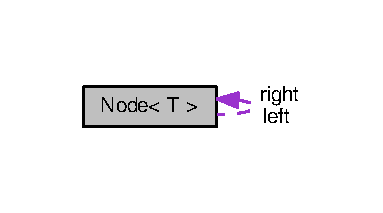
\includegraphics[width=184pt]{class_node__coll__graph}
\end{center}
\end{figure}
\subsection*{Public Member Functions}
\begin{DoxyCompactItemize}
\item 
\hyperlink{class_node_aa72a44d0679a17d33d7a6f2b41790125}{Node} (T value)
\begin{DoxyCompactList}\small\item\em Public constructor for creating new nodes It assigns value to new node and sets pointers to N\+Ull, bf to 0 and height to 1. \end{DoxyCompactList}\item 
\hyperlink{class_node_ae923d0417581dd19784d55b901f0f7f0}{$\sim$\+Node} ()
\end{DoxyCompactItemize}
\subsection*{Public Attributes}
\begin{DoxyCompactItemize}
\item 
T \hyperlink{class_node_ac450c71a8677a38d306361f9ced518d3}{data}
\item 
\hyperlink{class_node}{Node} $\ast$ \hyperlink{class_node_a6596c7ac17ecafff5522310c0da3a828}{left}
\item 
\hyperlink{class_node}{Node} $\ast$ \hyperlink{class_node_a4009a1138f2f04372037fbec63406f11}{right}
\item 
int \hyperlink{class_node_aaf22ddd5e77fcf19eab893bb58924158}{bf}
\item 
int \hyperlink{class_node_a15b477d75fdc30cac4847dab9c954568}{height}
\end{DoxyCompactItemize}


\subsection{Detailed Description}
\subsubsection*{template$<$class T$>$\\*
class Node$<$ T $>$}

A\+VL \hyperlink{class_node}{Node} class. 

Class that represents \hyperlink{class_node}{Node} of A\+VL Tree. It contains 2 pointers left and right to another nodes, it\textquotesingle{}s balance factor (bf), height and data that depends on given data type (has to be compatrable). For now all data is public for simplicity. 

Definition at line 20 of file node.\+hpp.



\subsection{Constructor \& Destructor Documentation}
\index{Node@{Node}!Node@{Node}}
\index{Node@{Node}!Node@{Node}}
\subsubsection[{\texorpdfstring{Node(\+T value)}{Node(T value)}}]{\setlength{\rightskip}{0pt plus 5cm}template$<$class T$>$ {\bf Node}$<$ T $>$\+::{\bf Node} (
\begin{DoxyParamCaption}
\item[{T}]{value}
\end{DoxyParamCaption}
)\hspace{0.3cm}{\ttfamily [inline]}}\hypertarget{class_node_aa72a44d0679a17d33d7a6f2b41790125}{}\label{class_node_aa72a44d0679a17d33d7a6f2b41790125}


Public constructor for creating new nodes It assigns value to new node and sets pointers to N\+Ull, bf to 0 and height to 1. 


\begin{DoxyParams}{Parameters}
{\em value} & -\/ comparable value that node will contain. \\
\hline
\end{DoxyParams}


Definition at line 30 of file node.\+hpp.

\index{Node@{Node}!````~Node@{$\sim$\+Node}}
\index{````~Node@{$\sim$\+Node}!Node@{Node}}
\subsubsection[{\texorpdfstring{$\sim$\+Node()}{~Node()}}]{\setlength{\rightskip}{0pt plus 5cm}template$<$class T$>$ {\bf Node}$<$ T $>$\+::$\sim${\bf Node} (
\begin{DoxyParamCaption}
{}
\end{DoxyParamCaption}
)\hspace{0.3cm}{\ttfamily [inline]}}\hypertarget{class_node_ae923d0417581dd19784d55b901f0f7f0}{}\label{class_node_ae923d0417581dd19784d55b901f0f7f0}
To avoid memory leaks, destructor deletes object\textquotesingle{}s left and right nodes 

Definition at line 33 of file node.\+hpp.



\subsection{Member Data Documentation}
\index{Node@{Node}!bf@{bf}}
\index{bf@{bf}!Node@{Node}}
\subsubsection[{\texorpdfstring{bf}{bf}}]{\setlength{\rightskip}{0pt plus 5cm}template$<$class T$>$ int {\bf Node}$<$ T $>$\+::bf}\hypertarget{class_node_aaf22ddd5e77fcf19eab893bb58924158}{}\label{class_node_aaf22ddd5e77fcf19eab893bb58924158}
Balance factor 

Definition at line 43 of file node.\+hpp.

\index{Node@{Node}!data@{data}}
\index{data@{data}!Node@{Node}}
\subsubsection[{\texorpdfstring{data}{data}}]{\setlength{\rightskip}{0pt plus 5cm}template$<$class T$>$ T {\bf Node}$<$ T $>$\+::data}\hypertarget{class_node_ac450c71a8677a38d306361f9ced518d3}{}\label{class_node_ac450c71a8677a38d306361f9ced518d3}
Comparable data contained in this node 

Definition at line 36 of file node.\+hpp.

\index{Node@{Node}!height@{height}}
\index{height@{height}!Node@{Node}}
\subsubsection[{\texorpdfstring{height}{height}}]{\setlength{\rightskip}{0pt plus 5cm}template$<$class T$>$ int {\bf Node}$<$ T $>$\+::height}\hypertarget{class_node_a15b477d75fdc30cac4847dab9c954568}{}\label{class_node_a15b477d75fdc30cac4847dab9c954568}
Height of this node in the tree 

Definition at line 46 of file node.\+hpp.

\index{Node@{Node}!left@{left}}
\index{left@{left}!Node@{Node}}
\subsubsection[{\texorpdfstring{left}{left}}]{\setlength{\rightskip}{0pt plus 5cm}template$<$class T$>$ {\bf Node}$\ast$ {\bf Node}$<$ T $>$\+::left}\hypertarget{class_node_a6596c7ac17ecafff5522310c0da3a828}{}\label{class_node_a6596c7ac17ecafff5522310c0da3a828}
Pointers for left and right nodes 

Definition at line 39 of file node.\+hpp.

\index{Node@{Node}!right@{right}}
\index{right@{right}!Node@{Node}}
\subsubsection[{\texorpdfstring{right}{right}}]{\setlength{\rightskip}{0pt plus 5cm}template$<$class T$>$ {\bf Node}$\ast$ {\bf Node}$<$ T $>$\+::right}\hypertarget{class_node_a4009a1138f2f04372037fbec63406f11}{}\label{class_node_a4009a1138f2f04372037fbec63406f11}


Definition at line 40 of file node.\+hpp.



The documentation for this class was generated from the following file\+:\begin{DoxyCompactItemize}
\item 
/home/kacper/\+Pulpit/\+P\+A\+M\+S\+I -\/ Projekty/\+Projekt 1/prj/inc/\hyperlink{node_8hpp}{node.\+hpp}\end{DoxyCompactItemize}

\chapter{File Documentation}
\hypertarget{additional_functions_8hpp}{}\section{/home/kacper/\+Pulpit/\+P\+A\+M\+SI -\/ Projekty/\+Projekt 1/prj/inc/additional\+Functions.hpp File Reference}
\label{additional_functions_8hpp}\index{/home/kacper/\+Pulpit/\+P\+A\+M\+S\+I -\/ Projekty/\+Projekt 1/prj/inc/additional\+Functions.\+hpp@{/home/kacper/\+Pulpit/\+P\+A\+M\+S\+I -\/ Projekty/\+Projekt 1/prj/inc/additional\+Functions.\+hpp}}
{\ttfamily \#include $<$iostream$>$}\\*
{\ttfamily \#include $<$cstdlib$>$}\\*
{\ttfamily \#include $<$ctime$>$}\\*
{\ttfamily \#include \char`\"{}A\+V\+L\+\_\+\+Tree.\+hpp\char`\"{}}\\*
Include dependency graph for additional\+Functions.\+hpp\+:
\nopagebreak
\begin{figure}[H]
\begin{center}
\leavevmode
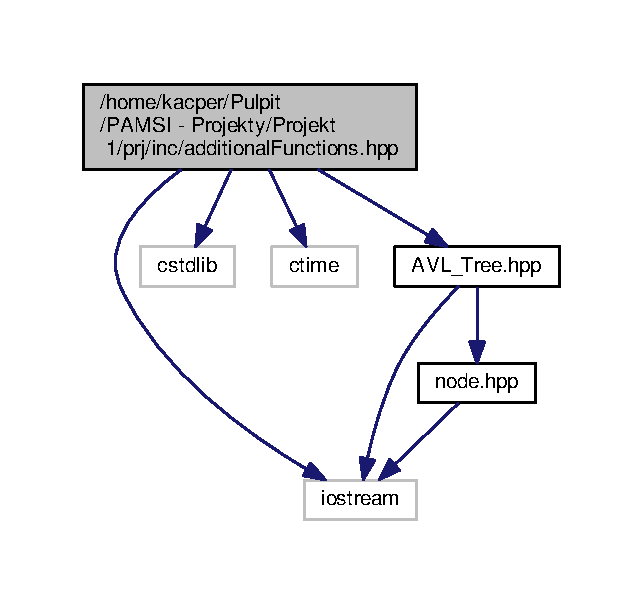
\includegraphics[width=309pt]{additional_functions_8hpp__incl}
\end{center}
\end{figure}
This graph shows which files directly or indirectly include this file\+:
\nopagebreak
\begin{figure}[H]
\begin{center}
\leavevmode
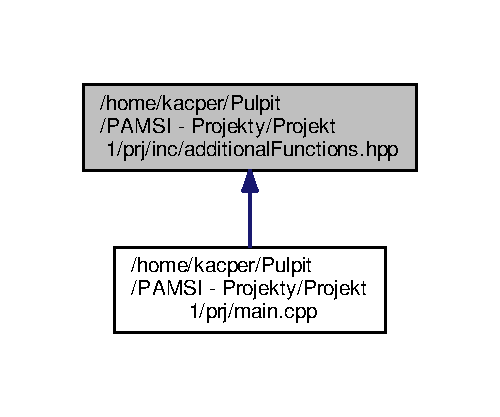
\includegraphics[width=240pt]{additional_functions_8hpp__dep__incl}
\end{center}
\end{figure}
\subsection*{Functions}
\begin{DoxyCompactItemize}
\item 
void \hyperlink{additional_functions_8hpp_aba5bd9067aa6f261123165a337c7957d}{show\+Menu} ()
\begin{DoxyCompactList}\small\item\em Function that shows menu. \end{DoxyCompactList}\item 
void \hyperlink{additional_functions_8hpp_aa0eaf0dfa340d7c9b88a540455bd401e}{quick\+Temp\+Tree\+Test} ()
\begin{DoxyCompactList}\small\item\em Function that do quick test of A\+VL Tree. \end{DoxyCompactList}\end{DoxyCompactItemize}


\subsection{Detailed Description}
This file contains functions for main program 

\subsection{Function Documentation}
\index{additional\+Functions.\+hpp@{additional\+Functions.\+hpp}!quick\+Temp\+Tree\+Test@{quick\+Temp\+Tree\+Test}}
\index{quick\+Temp\+Tree\+Test@{quick\+Temp\+Tree\+Test}!additional\+Functions.\+hpp@{additional\+Functions.\+hpp}}
\subsubsection[{\texorpdfstring{quick\+Temp\+Tree\+Test()}{quickTempTreeTest()}}]{\setlength{\rightskip}{0pt plus 5cm}void quick\+Temp\+Tree\+Test (
\begin{DoxyParamCaption}
{}
\end{DoxyParamCaption}
)}\hypertarget{additional_functions_8hpp_aa0eaf0dfa340d7c9b88a540455bd401e}{}\label{additional_functions_8hpp_aa0eaf0dfa340d7c9b88a540455bd401e}


Function that do quick test of A\+VL Tree. 

This function does basic test of A\+VL Tree methods using random integers 

Definition at line 44 of file additional\+Functions.\+hpp.

\index{additional\+Functions.\+hpp@{additional\+Functions.\+hpp}!show\+Menu@{show\+Menu}}
\index{show\+Menu@{show\+Menu}!additional\+Functions.\+hpp@{additional\+Functions.\+hpp}}
\subsubsection[{\texorpdfstring{show\+Menu()}{showMenu()}}]{\setlength{\rightskip}{0pt plus 5cm}void show\+Menu (
\begin{DoxyParamCaption}
{}
\end{DoxyParamCaption}
)}\hypertarget{additional_functions_8hpp_aba5bd9067aa6f261123165a337c7957d}{}\label{additional_functions_8hpp_aba5bd9067aa6f261123165a337c7957d}


Function that shows menu. 

Function that shows menu to an user, within itself it uses std namespace. 

Definition at line 21 of file additional\+Functions.\+hpp.


\hypertarget{_a_v_l___tree_8hpp}{}\section{/home/kacper/\+Pulpit/\+P\+A\+M\+SI -\/ Projekty/\+Projekt 1/prj/inc/\+A\+V\+L\+\_\+\+Tree.hpp File Reference}
\label{_a_v_l___tree_8hpp}\index{/home/kacper/\+Pulpit/\+P\+A\+M\+S\+I -\/ Projekty/\+Projekt 1/prj/inc/\+A\+V\+L\+\_\+\+Tree.\+hpp@{/home/kacper/\+Pulpit/\+P\+A\+M\+S\+I -\/ Projekty/\+Projekt 1/prj/inc/\+A\+V\+L\+\_\+\+Tree.\+hpp}}
{\ttfamily \#include $<$iostream$>$}\\*
{\ttfamily \#include \char`\"{}node.\+hpp\char`\"{}}\\*
Include dependency graph for A\+V\+L\+\_\+\+Tree.\+hpp\+:
\nopagebreak
\begin{figure}[H]
\begin{center}
\leavevmode
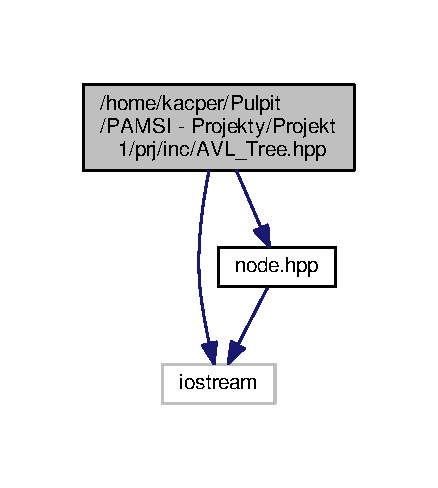
\includegraphics[width=210pt]{_a_v_l___tree_8hpp__incl}
\end{center}
\end{figure}
This graph shows which files directly or indirectly include this file\+:
\nopagebreak
\begin{figure}[H]
\begin{center}
\leavevmode
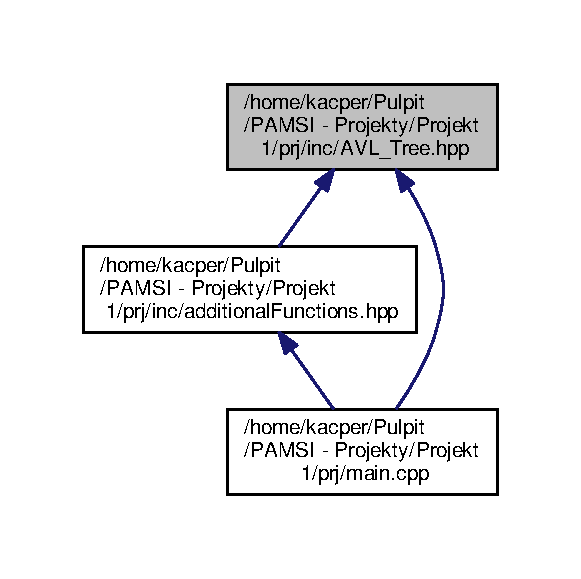
\includegraphics[width=279pt]{_a_v_l___tree_8hpp__dep__incl}
\end{center}
\end{figure}
\subsection*{Classes}
\begin{DoxyCompactItemize}
\item 
class \hyperlink{class_a_v_l___tree}{A\+V\+L\+\_\+\+Tree$<$ T $>$}
\begin{DoxyCompactList}\small\item\em A\+VL Tree class. \end{DoxyCompactList}\end{DoxyCompactItemize}


\subsection{Detailed Description}
This file contains template class \hyperlink{class_a_v_l___tree}{A\+V\+L\+\_\+\+Tree}, it\textquotesingle{}s constructor, destructor, properties and methods. 
\hypertarget{logger_8hpp}{}\section{/home/kacper/\+Pulpit/\+P\+A\+M\+SI -\/ Projekty/\+Projekt 1/prj/inc/logger.hpp File Reference}
\label{logger_8hpp}\index{/home/kacper/\+Pulpit/\+P\+A\+M\+S\+I -\/ Projekty/\+Projekt 1/prj/inc/logger.\+hpp@{/home/kacper/\+Pulpit/\+P\+A\+M\+S\+I -\/ Projekty/\+Projekt 1/prj/inc/logger.\+hpp}}
{\ttfamily \#include $<$iostream$>$}\\*
{\ttfamily \#include $<$fstream$>$}\\*
{\ttfamily \#include $<$cstring$>$}\\*
Include dependency graph for logger.\+hpp\+:
\nopagebreak
\begin{figure}[H]
\begin{center}
\leavevmode
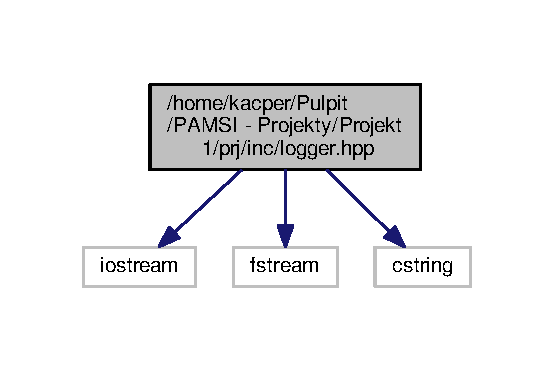
\includegraphics[width=266pt]{logger_8hpp__incl}
\end{center}
\end{figure}
This graph shows which files directly or indirectly include this file\+:
\nopagebreak
\begin{figure}[H]
\begin{center}
\leavevmode
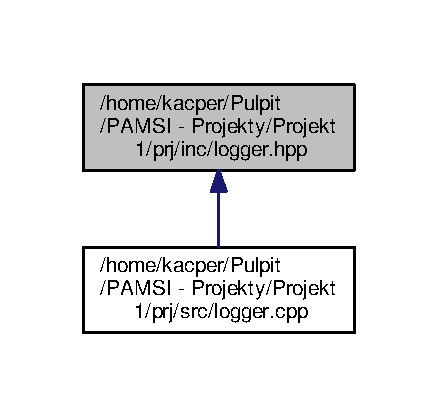
\includegraphics[width=210pt]{logger_8hpp__dep__incl}
\end{center}
\end{figure}
\subsection*{Classes}
\begin{DoxyCompactItemize}
\item 
class \hyperlink{class_logger}{Logger}
\end{DoxyCompactItemize}

\hypertarget{node_8hpp}{}\section{/home/kacper/\+Pulpit/\+P\+A\+M\+SI -\/ Projekty/\+Projekt 1/prj/inc/node.hpp File Reference}
\label{node_8hpp}\index{/home/kacper/\+Pulpit/\+P\+A\+M\+S\+I -\/ Projekty/\+Projekt 1/prj/inc/node.\+hpp@{/home/kacper/\+Pulpit/\+P\+A\+M\+S\+I -\/ Projekty/\+Projekt 1/prj/inc/node.\+hpp}}
{\ttfamily \#include $<$iostream$>$}\\*
Include dependency graph for node.\+hpp\+:
\nopagebreak
\begin{figure}[H]
\begin{center}
\leavevmode
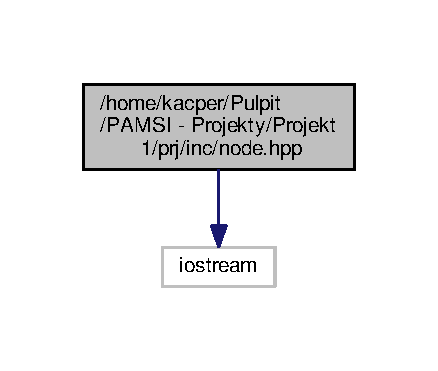
\includegraphics[width=210pt]{node_8hpp__incl}
\end{center}
\end{figure}
This graph shows which files directly or indirectly include this file\+:
\nopagebreak
\begin{figure}[H]
\begin{center}
\leavevmode
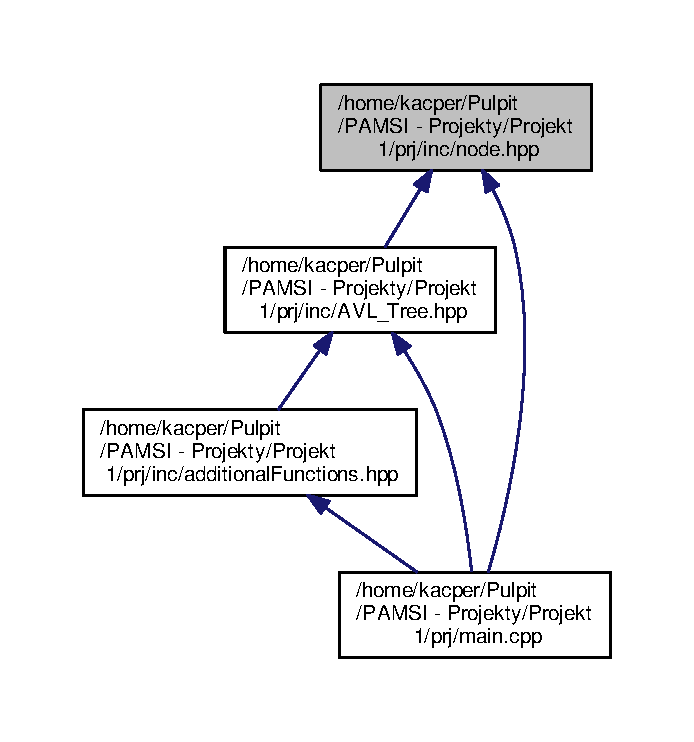
\includegraphics[width=333pt]{node_8hpp__dep__incl}
\end{center}
\end{figure}
\subsection*{Classes}
\begin{DoxyCompactItemize}
\item 
class \hyperlink{class_node}{Node$<$ T $>$}
\begin{DoxyCompactList}\small\item\em A\+VL \hyperlink{class_node}{Node} class. \end{DoxyCompactList}\end{DoxyCompactItemize}


\subsection{Detailed Description}
This file contains template class \hyperlink{class_node}{Node}, it\textquotesingle{}s constructor and destructor + it\textquotesingle{}s properties 
\hypertarget{main_8cpp}{}\section{/home/kacper/\+Pulpit/\+P\+A\+M\+SI -\/ Projekty/\+Projekt 1/prj/main.cpp File Reference}
\label{main_8cpp}\index{/home/kacper/\+Pulpit/\+P\+A\+M\+S\+I -\/ Projekty/\+Projekt 1/prj/main.\+cpp@{/home/kacper/\+Pulpit/\+P\+A\+M\+S\+I -\/ Projekty/\+Projekt 1/prj/main.\+cpp}}
{\ttfamily \#include $<$cstring$>$}\\*
{\ttfamily \#include \char`\"{}inc/node.\+hpp\char`\"{}}\\*
{\ttfamily \#include \char`\"{}inc/\+A\+V\+L\+\_\+\+Tree.\+hpp\char`\"{}}\\*
{\ttfamily \#include \char`\"{}inc/additional\+Functions.\+hpp\char`\"{}}\\*
Include dependency graph for main.\+cpp\+:
\nopagebreak
\begin{figure}[H]
\begin{center}
\leavevmode
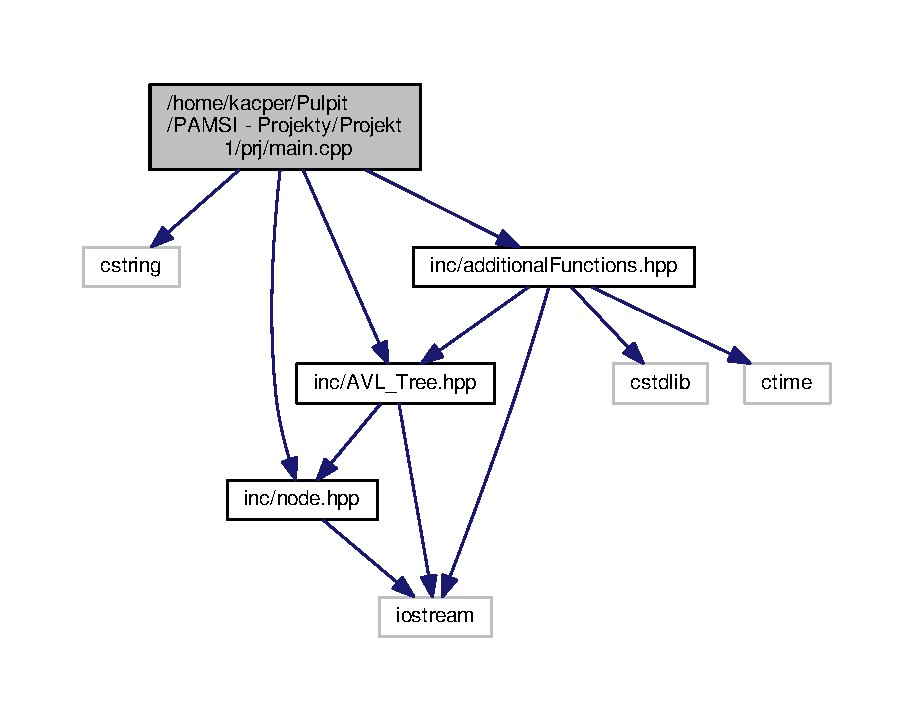
\includegraphics[width=350pt]{main_8cpp__incl}
\end{center}
\end{figure}
\subsection*{Functions}
\begin{DoxyCompactItemize}
\item 
int \hyperlink{main_8cpp_ae66f6b31b5ad750f1fe042a706a4e3d4}{main} ()
\end{DoxyCompactItemize}


\subsection{Function Documentation}
\index{main.\+cpp@{main.\+cpp}!main@{main}}
\index{main@{main}!main.\+cpp@{main.\+cpp}}
\subsubsection[{\texorpdfstring{main()}{main()}}]{\setlength{\rightskip}{0pt plus 5cm}int main (
\begin{DoxyParamCaption}
{}
\end{DoxyParamCaption}
)}\hypertarget{main_8cpp_ae66f6b31b5ad750f1fe042a706a4e3d4}{}\label{main_8cpp_ae66f6b31b5ad750f1fe042a706a4e3d4}


Definition at line 6 of file main.\+cpp.


\hypertarget{logger_8cpp}{}\section{/home/kacper/\+Pulpit/\+P\+A\+M\+SI -\/ Projekty/\+Projekt 1/prj/src/logger.cpp File Reference}
\label{logger_8cpp}\index{/home/kacper/\+Pulpit/\+P\+A\+M\+S\+I -\/ Projekty/\+Projekt 1/prj/src/logger.\+cpp@{/home/kacper/\+Pulpit/\+P\+A\+M\+S\+I -\/ Projekty/\+Projekt 1/prj/src/logger.\+cpp}}
{\ttfamily \#include \char`\"{}../inc/logger.\+hpp\char`\"{}}\\*
Include dependency graph for logger.\+cpp\+:
\nopagebreak
\begin{figure}[H]
\begin{center}
\leavevmode
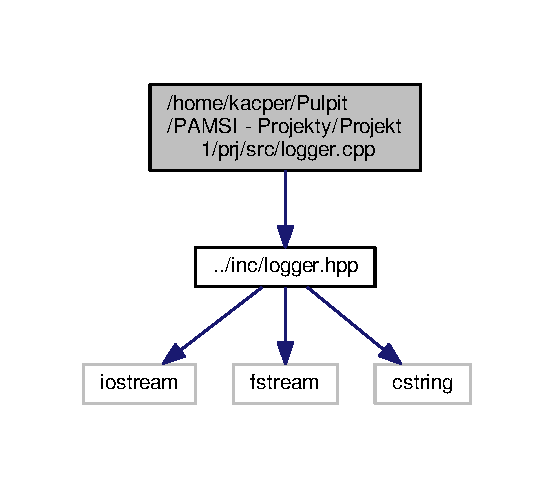
\includegraphics[width=266pt]{logger_8cpp__incl}
\end{center}
\end{figure}

%--- End generated contents ---

% Index
\backmatter
\newpage
\phantomsection
\clearemptydoublepage
\addcontentsline{toc}{chapter}{Index}
\printindex

\end{document}
